Das Klimasystem ist ein komplexes und hoch-dimensionales System. Dieses durch ein Modell berechenbar zu machen ist dementsprechend schwierig und bedarf einiger Abstraktionen. Laut Definition (vgl. Stachowiak in \cite{stachowiak}) sollen Modelle nicht alle Attribute des abgebildeten Systems übernehmen, sondern vielmehr eine Vereinfachung dessen sein mit einer kleinst-möglichen und aber notwendig großen Komplexität. Auf Klimamodelle bezogen, bedeutet dies, dass man nicht alle einzelnen Bausteine des Klimas durch das Modell abbilden soll, sondern manche Bausteine durch Parameter und Annäherungen abgebildet werden müssen. Ein globales Klimamodell (GCM) liefert im generellen recht gute Aussagen über die Entwicklung des globalen Klimas, jedoch beruhen diese Ozean-Atmosphären gekoppelten Zirkulationsmodelle, auf einer Parametrisierung der Konvektion, da diese im relativ groben Raster eines GCM nicht simuliert werden kann. Dadurch können grobe Fehler entstehen. (vgl. Stevens \& Bony in \cite{stevensbony}). Jedoch ist aufgrund der Rechenkosten und Rechenzeit eine solche Herangehensweise mit parametrisierter Konvektion im Simulieren großflächiger (globaler) Klimamodelle  unumgänglich. Großflächige Prozesse des Klimas wie z.B. der polare Jet, die nordatlantischen Stürme oder auch die stationären planetaren Wellen werden jedoch in den Modellen simuliert.\\
Viele GCMs bzw. deren Simulationsergebnisse müssen aufgrund der Parametrisierung und auch anderer Probleme wie z.B. der Darstellung der Topographie in niedriger Auflösung korrigiert werden. Dadurch sind diese GCMs eine starke Fehlerquelle in regionalen Klimamodellen (vgl. \cite{woollings_2013}).\\
Um akkurate Aussagen über die regionale Klimaveränderung  basierend auf GCMs zu tätigen, muss das globale Klimamodell auf die entsprechende Region downgescaled werden. Da auf der regionalen Ebene die Ortographie (wie z.B die Alpen), die flache Konvektion, die zur Tiefen-Konvektion wird und die lokalen Kältepools große Auswirkungen auf die Wettererscheinungen haben, müssen diese entweder statistisch parametrisiert oder dynamisch berechnet werden. Diese Vereinfachungen sind auch eine große Fehlerquelle für die regionalen Klimamodelle (vgl. \cite{maraun_2010,casanueva_2013}).\\
%Zudem kommen noch etwaige Rückkopplungen des regionalen Klimas auf das Globale hinzu, was zu einer weiteren Fehlerquelle führen kann. Wie man in der Publikation von Teixera et al.\cite{teixeracardoso} und Chen et al.\cite{chenshuyi} lesen kann hat die flache Konvektion durch ihre starke Rückwirkungen auf die Tiefen-Konvektion auch eine Auswirkung auf das globale Klima, wie es z.B. gut anhand der Tropen und der Madden-Julian Oszillation zu erkennen ist, wo aus flacher Konvektion Tiefen-Konvektoin wird und daraus sich großflächige Wettererscheinungen bilden.
Zudem sollte hier angeführt werden, dass auch die Auflösung von gegenwärtigen Klimamodelle nicht immer ausreichend ist: z.B. können Turbulenzen und andere atmosphärische Mikroprozesse häufig nicht von der derzeitigen Maschenweite der Simulationsgitter vollends erfasst und müssen, um grobe Fehler zu vermeiden, statistisch und dynamisch kombiniert downgescaled werden (vgl. \cite{marauntowards}).\\
Als letzte große Fehlerquelle für regionale- und auch globale Klimamodelle sollte die interne Variabilität des Klimas angeführt werden: Alle externen Klimaeinflüsse wie z.B. der Mensch oder auch vulkanische und astronomische Erscheinungen führen zu einer Klimareaktion, welche von internen Klimafluktuationen überlagert wird. Da diese Klimaeinflüsse nicht modelliert werden können ist es auch nicht möglich ein Klimamodell zu entwickeln, welches nicht von zufälligen Fluktuationen dominiert ist (siehe \cite{maraun_value}, Seite 3).\\
\begin{figure}[h]
	\centering
	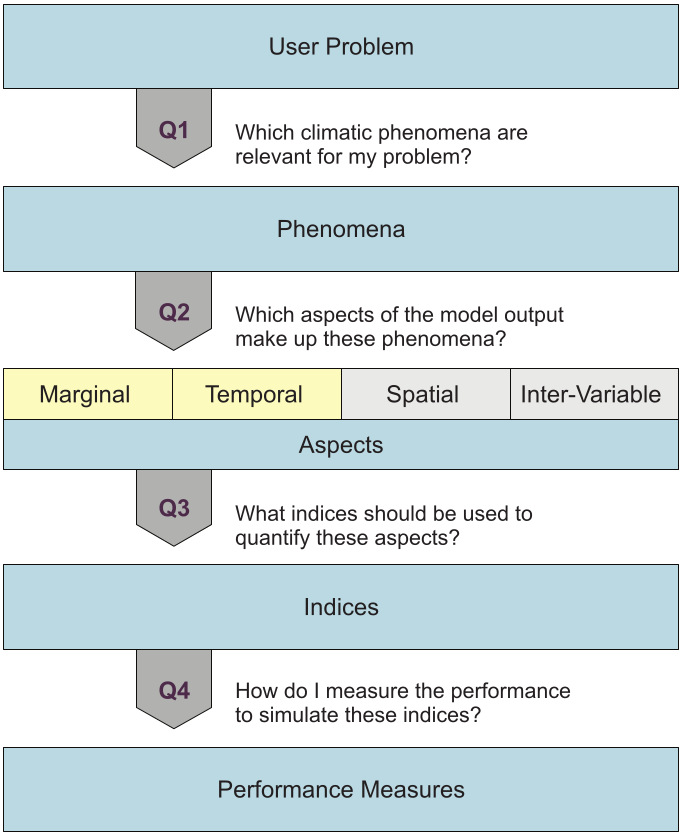
\includegraphics[width=0.5\textwidth]{VALUE.png}
	\caption{Baumstruktur, um eine geeignete Evaluationsmethode zu finden \cite{maraun_value}}
	\label{fig:value}
\end{figure}

Um eine geeignete Evaluierungsmethode zu finden, halte ich mich an die Herangehensweise aus Abb. \ref{fig:value}:
\begin{itemize}
	\item Q1: Starkregenereignisse, und Übereinstimmung von Niederschlagsmustern
	\item Q2:
		\subitem{*} Marginal: Intensität
		\subitem{*} Temporal: Jahreszeit bzw. Dauer der Erscheinungen.
		\subitem{*} Spatial: Gewitterzellen sind auf kleinen Arealen zu finden (in den Alpen)
		\subitem{*} Inter-Variable: Temperatur als Begleiterscheinung bei Gewittern.
	\item Q3: Mittelwert der Niederschläge, 99. Quantile, Jahreszeiten, Temperatur-Niederschlagskorrelation, Übereinstimmung der Verteilungskurven und damit dem BIAS der Kurven, räumliche Übereinstimmung mit den Beobachtungsdaten.
	\item Q4: BIAS und relative Fehler (zu den Beobachtungsdaten)
\end{itemize}

Um nun die beiden regionalen Klimamodelle möglichst allgemein miteinander zu vergleichen werde ich sie über den Mittelwert des Niederschlags, das 99. Quantil über alle zehn Jahre und das 99. Quantil in den vier Jahreszeiten vergleichen. In allen Fällen soll besonders auf die örtliche Verteilung Wert gelegt werden, da dies ein ausschlaggebender Punkt für die Vorhersagekraft regionaler Klimamodelle ist.



